%% skycell --- manuscript for Astronomy and Computing (Elsevier).
%%
%% Build from paper/:   make ac     (needs elsarticle.cls, in TeX Live)
%% The text is ../content.tex, shared with the A&A version (../body.tex);
%% this file holds only the journal's own front and back matter.
%% Highlights go in as a separate file at submission: highlights.txt.
\documentclass[preprint,12pt]{elsarticle}

\usepackage{graphicx}
\usepackage{amsmath}
\usepackage{amssymb}
\usepackage{url}
\usepackage[bookmarks=false,colorlinks=true,linkcolor=black,citecolor=black,urlcolor=blue]{hyperref}

%% the A&A class's astronomical units, and the section-reference word
\newcommand{\arcsec}{\ensuremath{^{\prime\prime}}}
\newcommand{\arcmin}{\ensuremath{^{\prime}}}
\newcommand{\degr}{\ensuremath{^{\circ}}}
\newcommand{\Sect}{Section}
\usepackage{rotating}
\newenvironment{widetable}{\begin{sidewaystable}}{\end{sidewaystable}}
\emergencystretch=2em

\journal{Astronomy and Computing}

\begin{document}

\begin{frontmatter}

\title{skycell: a cost-based HEALPix index for sky positions in PostgreSQL}

\author[skao]{Jes\'us Salgado\corref{cor}}
\ead{jesus.salgado@skao.int}
\author[skao]{Michele Delli Veneri}
\ead{michele.delliveneri@skao.int}
\cortext[cor]{Corresponding author}
\affiliation[skao]{organization={SKA Observatory},
  addressline={Jodrell Bank, Lower Withington},
  city={Macclesfield},
  postcode={SK11 9FT},
  country={United Kingdom}}

\begin{abstract}
Astronomical archives answer positional queries from relational databases, and in
PostgreSQL two extensions dominate: Q3C, which keys sources by a cube quad-tree index in
a B-tree, and pgSphere, which stores spherical geometry in a GiST tree and also indexes
regions. We present \texttt{skycell}, a PostgreSQL extension that keeps the integer key
and the B-tree yet answers cones, polygons, cross-matches and stored footprints in the
archives' own ADQL vocabulary. Positions are keyed by their order-29 HEALPix cell, and a
query region is covered by cells whose depth is chosen by a cost model: the price of an
extra index range against the false-positive rows it removes, with local source density
read from the histogram PostgreSQL already keeps. Cones and cross-matches are answered by
a planner custom scan that walks the covering's ranges, polygons by a rewrite into range
conditions, and stored regions by a GiST operator class. Coverings are validated by
brute force over millions of points. In randomized paired trials on PostgreSQL 18.6 with
10- and 50-million-row catalogues, including real Gaia DR3 positions, \texttt{skycell}
is faster than pgSphere at every cone radius from 1\arcsec\ to 3\degr, by 4--33\% with a
warm cache and up to 2.7 times cold. It cross-matches 20--33\% faster than Q3C's
\texttt{q3c\_join} and three times faster than pgSphere, and answers convex polygons
2.7--4.4 times faster than pgSphere, from an index a third the size. One index serving
points, regions and cross-matches through ADQL makes \texttt{skycell} a strong default
for an archive's positional layer.
\end{abstract}

\begin{highlights}
\item A HEALPix B-tree index for PostgreSQL answering cones, polygons and cross-matches
\item A cost model sets each covering's depth from local density and index range price
\item Faster than pgSphere at every cone radius from 1 arcsec to 3 deg, real Gaia DR3 too
\item Cross-matches 20--33\% faster than q3c\_join, from an index a third of pgSphere's size
\item Speaks ADQL; one column holds circles and polygons, read and written as IVOA STC-S
\end{highlights}

\begin{keyword}
Astronomical databases \sep Spatial indexing \sep HEALPix \sep PostgreSQL \sep
Cross-matching \sep Virtual Observatory \sep ADQL
\end{keyword}

\end{frontmatter}

%% The paper's shared text, from the Introduction to the Conclusions.
%% Input by body.tex (A&A) and ac/skycell-ac.tex (Astronomy and Computing);
%% each defines \Sect ("Sect." or "Section") and may define widetable, the
%% float for a table wider than a column (table* by default).
\makeatletter
\@ifundefined{widetable}{\newenvironment{widetable}{\begin{table*}}{\end{table*}}}{}
\makeatother

\section{Introduction}

Almost every question asked of an astronomical archive is positional: what is within
this cone, which observations cover this field, which of my sources match that
catalogue. In the Virtual Observatory these arrive as ADQL \citep{adql} through the
Table Access Protocol \citep{tap}, and the service must answer them with an index. The
scale is set by archives already in operation: the ESA Gaia Archive
\citep{gaiaarchive1, gaiaarchive2} serves order $10^9$ sources and lists cross-match
among its server-side capabilities.

Two PostgreSQL extensions carry most of this traffic. Q3C \citep{q3c} projects the
sphere onto a cube, subdivides each face with a quad-tree, and numbers the cells along a
space-filling curve, so each source is one 64-bit integer in a B-tree. pgSphere
\citep{pgsphere} adds spherical types indexed with GiST over bounding volumes, so
regions can be stored and queried as data. Neither idea is new -- the Hierarchical
Triangular Mesh \citep{htm} keyed positions by a subdivided polyhedron, and the zones
algorithm \citep{zones} arranged a catalogue for cross-matching -- but catalogues have
grown, and most queries now arrive through a generated layer \citep[e.g.][]{dachs}
rather than being hand-written.

The two designs trade off: a linear key in a B-tree is compact and cheap to probe, but a
region must first become a set of key ranges, whose quality depends on how finely the
region is cut; a tree of bounding volumes needs no such step but has larger, overlapping
keys. This paper presents \texttt{skycell}, which keeps the integer key and treats the
cut as a cost question answered from two quantities the database already knows: local
source density and the price of an index range. Section~\ref{sec:method} describes the
index, \Sect~\ref{sec:region-index} the region index, \Sect~\ref{sec:validation} its
correctness, \Sect~\ref{sec:adql} the ADQL surface, \Sect~\ref{sec:tests} the
performance comparison, and \Sect~\ref{sec:conclusions} concludes.

\section{The index}
\label{sec:method}

\subsection{An equal-area integer key}
\label{sec:key}

A position is keyed by its order-29 HEALPix cell in the nested scheme \citep{healpix}
($12\cdot4^{29}\approx3.5\times10^{18}$ cells of about 0.4\,mas), stored as a 64-bit
integer, so a B-tree orders keys along the HEALPix curve. Three properties follow. Cells
are \emph{nested}: the order-29 descendants of a cell $p$ at order $k$ are exactly the
contiguous interval
\begin{equation}
  \bigl[\, p\cdot 4^{\,29-k},\; (p+1)\cdot 4^{\,29-k} - 1 \,\bigr],
  \label{eq:interval}
\end{equation}
so a region covered by cells of any orders becomes a union of integer intervals a
B-tree answers with range scans. Cells are \emph{equal area}, so keys per interval are
proportional to source density per solid angle: the \texttt{ANALYZE} histogram is a
crowding map with no extra machinery (\Sect~\ref{sec:density}). And cells are
\emph{standard} -- the numbering underlies Gaia's \texttt{source\_id} \citep{gaia} and
IVOA MOC maps \citep{moc} -- so keys, coverings and footprints are interoperable.

\subsection{Coverings decided by cost}
\label{sec:cost}

A query region is covered by cells whose union contains it; the covering becomes range
conditions on the key, and rows inside the covering but outside the region are removed
by an exact test. Cutting finer means fewer false positives and more ranges. With cells
of size $s$ covering a region of radius $r$ and local source density $\rho$,
\begin{equation}
  C(s) = n_{\rm ranges}(s)\,c_{\rm range} + \rho\,\bigl(A_{\rm cover}(s) - A_{\rm region}\bigr),
  \label{eq:cost}
\end{equation}
both terms in rows: the second is the expected false positives, and $c_{\rm range}$
converts one additional index range into the false-positive rows it is worth avoiding.
A covering follows the region's boundary, so for $s\ll r$ the ranges grow as $r/s$
while the wasted area grows as the perimeter times $s$; writing
$A_{\rm cover}\simeq\pi(r+\beta s)^2$ and $n_{\rm ranges}\simeq\gamma r/s$ and
minimising Eq.~(\ref{eq:cost}) gives
\begin{equation}
  s_\star = \sqrt{\frac{\gamma\,c_{\rm range}}{2\pi\beta\,\rho}},
  \label{eq:sstar}
\end{equation}
independent of region size: sky density and range price alone decide how finely to cut.
For $s\gtrsim r$ the balance differs, so the implementation evaluates
Eq.~(\ref{eq:cost}) at all 30 orders and takes the cheapest. The same $0.25\degr$ cone
illustrates both regimes: at high Galactic latitude, 11 sources leave almost nothing to
exclude, so the model buys one range of large cells (5.6 times the cone's area); in the
bulge, 1183 sources make false positives cost more than extra ranges, so it cuts two
orders deeper (8 ranges, 1.3 times the area). Two guards keep the model safe against its
own inputs: a partly covered cell may not exceed 64 times the region's area, bounding
the damage from a cluster the histogram underestimates, and gaps between ranges are
merged when the rows they hold cost less than the range they save.

\paragraph{The range price.}
\label{sec:calib}
$c_{\rm range}$ is not a free parameter: it is the ratio of two costs PostgreSQL already
models, one more index range against one false-positive row. A range costs a B-tree
descent plus two pages -- the leaf it lands on and the heap page where the scan stops
running sequentially -- and a false row its index entry, heap tuple, exact test and its
share of a heap page, each page priced at $p = f\,50\,c_{\rm op} + (1-f)\,c_{\rm page}$
by where it is expected to come from:
\begin{equation}
  c_{\rm range} = \frac{\lceil\log_2 N\rceil\,c_{\rm op} + 50(H+1)\,c_{\rm op} + 2p}
    {c_{\rm tuple} + c_{\rm itup} + k\,c_{\rm op} + p/n_{\rm pp}},
  \label{eq:crange}
\end{equation}
with $N$ rows, $H$ the B-tree height, $n_{\rm pp}$ rows per heap page, $k$ the
operators of the exact test, the $c$ the planner's own cost factors, and $f=\min(1,\mathrm{shared\_buffers}/\mathrm{relpages})$
the fraction of the relation the buffer pool can hold. For a 10-million-row catalogue
this is 34 rows with the relation in the pool and 87 with none of it there; a wide
observation row, with fewer rows per page, is cut finer. The cost curve is flat near its
optimum -- across four decades of $c_{\rm range}$ the median query time moves by under
25\% between 3 and 300, and the order chosen is within about 3\% of the best -- so
deriving the price per relation costs nothing in speed and leaves nothing to tune.

\paragraph{The density estimate.}
\label{sec:density}
\texttt{ANALYZE} stores, for the indexed expression, an equi-depth histogram of $B+1$
bounds $h_0<\dots<h_B$ such that each bucket holds about $N/B$ rows. Because the key is
an equal-area cell index, the rows in a key interval $[a,b]$ are estimated by linear
interpolation within the buckets it spans,
\begin{equation}
  \hat{n}(a,b) = \frac{N}{B}\sum_{i} \frac{\bigl|[a,b] \cap [h_i, h_{i+1})\bigr|}{h_{i+1}-h_i},
  \label{eq:hist}
\end{equation}
and the density in rows per steradian as
\begin{equation}
  \hat{\rho}(a,b) = \frac{\hat{n}(a,b)}{(b-a+1)\,A_{29}},
  \label{eq:rho}
\end{equation}
with $A_{29}$ the area of a leaf cell, evaluated over the cell containing the region's centre at the order whose cells are
about four times the region's size: large enough to hold a density, small enough to be
local. A cluster smaller than one bucket is averaged away, which the area guard bounds;
\Sect~\ref{sec:estimator} measures the estimate on real positions.

\paragraph{Classifying cells.}
\label{sec:classify}
A cell is classified against the region as inside, outside or straddling its boundary.
The outcomes are not symmetric: a cell wrongly called \emph{outside} silently loses
rows, while \emph{inside} and \emph{straddling} cells only produce a superset the exact
test trims. Only the outside decision therefore needs a bound. The one used is
\begin{equation}
  R_{\rm cell}(k,p) = \min\bigl(\mathrm{maxpixrad}(k),\;
    \max_{i}\, \angle(\mathbf{c}_{k,p}, \mathbf{v}_i)\bigr),
  \label{eq:rcell}
\end{equation}
with $\mathbf{c}_{k,p}$ the cell's centre, $\mathbf{v}_i$ its corners, and the first
term the analytic worst case of the reference HEALPix implementation. A cell is outside
a cone of centre $\mathbf{q}$ and radius $r$ when
$\angle(\mathbf{q},\mathbf{c}_{k,p})-R_{\rm cell}>r+\epsilon$ (per bounding half-space
for a polygon), with $\epsilon=2\times10^{-13}$\,rad covering accumulated floating-point
error, five orders of magnitude below the leaf cell. The inside test uses the cell's own
corners and edge midpoints, since optimism there costs false positives, never rows.

\subsection{Answering a query}
\label{sec:impl}
\label{sec:customscan}

The extension is written in C against the PostgreSQL server API, with a planner support
function on each spatial predicate. A cone -- \texttt{skycell\_cone}, the Q3C-shaped
\texttt{skycell\_join} and \texttt{skycell\_radial\_query}, or ADQL's own
\texttt{point <@ circle} -- is left as one clause whose selectivity the support function
supplies, and answered by a planner \emph{custom scan}: a path hook offers it wherever a
B-tree on the cell expression can serve the clause, costed as PostgreSQL costs the same
work. The node computes the covering and walks its ranges in one of two modes, chosen
from the column's correlation as PostgreSQL chooses between an index and a bitmap scan:
one index scan per range in cell order when the heap follows the cell order, or every
range's TIDs into one bitmap, each heap page read once, when it does not. Rows are
rechecked with the exact test. A cone whose centre comes from another relation's row --
a cross-match -- gets the same node parameterized by that row on the inner side of a
nested loop, each probe covered with the ranges its own cone needs; its row estimate is
measured at plan time on 32 sampled probes, since a density model cannot know that
cross-match targets sit on catalogue sources. Polygons and boxes are instead rewritten
before path generation into a disjunction of range conditions on the key plus the exact
test, whose selectivity the planner estimates from the same histogram. The density
model, index identity and coverings are cached per backend.

\paragraph{Ingestion and maintenance.} The index is an ordinary B-tree on an expression:
one 8-byte key per insert, no method-specific rebalancing. Because the covering reads
the histogram, statistics matter more than for a GiST index; the area guard bounds the
damage from a stale one, and \texttt{ANALYZE} on a 10-million-row catalogue takes about
a second.

\section{The region index}
\label{sec:region-index}

\paragraph{Regions as stored objects.}
\label{sec:moc}
\texttt{skyregion} is one type tagged by kind rather than a family of per-shape types, so
a single footprint column holds circles and polygons together -- as an ObsCore
\texttt{s\_region} column does, mixing single-pointing circles with polygons. pgSphere's
\texttt{scircle} and \texttt{spoly} are separate types, so a mixed-shape column needs two
columns in its place. A footprint can be covered by a few cells written in the MOC
standard's \texttt{NUNIQ} encoding and stored one per row in an ordinary B-tree; the
footprints containing a position are those whose cell is one of its ancestors, a short
list of equality lookups.

\paragraph{A GiST opclass family.}
\label{sec:gist-family}
A \texttt{skyregion} column can instead carry its own GiST index, serving \texttt{\&\&}
and both containment operators directly. Its default key is an axis-aligned 3D box
rounded outward to \texttt{float4} (24 bytes, pgSphere's own GiST representation),
sound because the recheck is exact whatever the key's precision: a looser box costs
false positives, never rows. A key of a few spherical caps, exact for a circle at any
radius, remains available for columns mixing very different region scales.

\section{Correctness}
\label{sec:validation}

\begin{quote}
\textbf{Proposition.} Let $R$ be a cone or convex polygon and let $\mathcal{C}$ be the
covering computed for it. If (i) every point of a HEALPix cell at order $k$ lies within
$\mathrm{maxpixrad}(k)$ of that cell's centre, and (ii) every angle computed by the
classification carries an absolute error below $\epsilon$, then every order-29 cell that
intersects $R$ lies in one of the ranges of $\mathcal{C}$.
\end{quote}

\emph{Proof sketch.} The descent starts from cells whose union is the whole sphere and,
at each step, keeps a cell, drops it, or replaces it by its four children, so the kept
union shrinks only where a cell is dropped, which happens only when it is classified
outside. By (i), every point of cell $(k,p)$ lies within $R_{\rm cell}$ of its centre,
so (ii) and the triangle inequality make
$\angle(\mathbf{q},\mathbf{c}_{k,p})-R_{\rm cell}>r+\epsilon$ sufficient for the whole
cell to miss the cone; the polygon case applies the same argument per bounding
half-space. Truncation (range cap, area guard, step budget) only stops refinement,
keeping a cell whole, so it cannot remove one either. $\square$

Condition (i) is a property of HEALPix (the reference $\mathrm{maxpixrad}$ is analytic;
verified over $1.6\times10^6$ sampled boundary points, largest observed ratio 0.9999);
(ii) is an assumption about floating-point arithmetic, with $\epsilon$ five orders of
magnitude above the plausible accumulated error. Because a missed cell silently loses
rows, the implementation is also checked by exhaustion: the HEALPix layer (known
centres, round trips at all 30 orders, nesting, equal area), and the covering against a
2-million-point clustered catalogue for cones to $120\degr$ and convex polygons, 30\,000
adversarial cones (poles, zone boundaries, face edges, radii 0.02\,mas--10\degr) and
7266 adversarial polygons with 869\,117 points -- all asserting zero false negatives.
SQL regression suites, run on PostgreSQL 16 and 18, require every indexed answer to
equal a sequential scan with the exact predicate, and the custom scan to return the same
rows as the range rewrite in both of its modes, for constant cones, cross-matches and
every spelling of the predicate.

\section{The ADQL surface}
\label{sec:adql}

The extension exposes ADQL's own vocabulary: types \texttt{skypos} and
\texttt{skyregion} and functions \texttt{point}, \texttt{circle}, \texttt{box},
\texttt{polygon}, \texttt{contains}, \texttt{intersects}, \texttt{distance},
\texttt{area}, \texttt{coord1}, \texttt{coord2} and \texttt{centroid}, so a translator
emits the standard's spelling rather than a dialect (Table~\ref{tab:ops}). The operator
\texttt{point <@ circle} is the indexable form of \texttt{CONTAINS}, answered by the
custom scan whether the circle is a constant or comes from another table's row, which
makes an ADQL cross-match as fast as the native one. \texttt{skyregion}'s text
representation is IVOA STC-S \citep{stc}, the syntax an ObsCore \texttt{s\_region}
column already carries, so such a column casts from and prints back as the archive's own
text. For SQL migrating from Q3C, \texttt{skycell\_radial\_query} and
\texttt{skycell\_join} take Q3C's argument lists unchanged. The IVOA UDF registry's
epoch-propagation and HEALPix functions are implemented with the rigorous propagation of
the Hipparcos catalogue \citep{hipparcos}, so a proper-motion-aware cone search is an
indexable cone widened by the largest motion of interest plus an exact test on the
propagated position.

\begin{table}
  \caption{What a translator emits for the ADQL constructs where the pgSphere-plus-Q3C
    pair and \texttt{skycell} differ most.}
  \label{tab:ops}
  \centering
  \footnotesize
  \begin{tabular}{@{}p{0.2\columnwidth} p{0.38\columnwidth} p{0.24\columnwidth}@{}}
    \hline\hline
    ADQL & pgSphere $+$ Q3C & skycell \\
    \hline
    \texttt{POINT}\allowbreak/\allowbreak\texttt{CIRCLE}\allowbreak/\allowbreak\texttt{POLYGON} &
      \texttt{spoint}\allowbreak/\allowbreak\texttt{scircle}\allowbreak/\allowbreak\texttt{spoly} &
      \texttt{point}\allowbreak/\allowbreak\texttt{circle}\allowbreak/\allowbreak\texttt{polygon} \\[2pt]
    \texttt{CONTAINS(}\allowbreak\texttt{POINT,}\allowbreak\ \texttt{CIRCLE)} &
      \texttt{q3c\_radial\_query} \emph{or}\allowbreak\ \texttt{pos <@ scircle} &
      \texttt{point <@ circle} \\[2pt]
    \texttt{INTERSECTS(}\allowbreak\texttt{r$_1$,}\allowbreak\texttt{r$_2$)} &
      \texttt{r$_1$ \&\& r$_2$} (no Q3C region type) &
      \texttt{r$_1$ \&\& r$_2$} \\[2pt]
    cross-match &
      \texttt{q3c\_join}, a separate function &
      \texttt{point <@ circle} in the join \\[2pt]
    \hline
  \end{tabular}
\end{table}

\section{Performance}
\label{sec:tests}

\subsection{Corpora, protocol and hosts}
\label{sec:corpora}
\label{sec:protocol}

Three 10-million-row catalogues answer the objections each previous one invites. The
\emph{designed} corpus is synthetic, with a density contrast resembling an optical
survey (35\% uniform, 45\% Galactic disk, 12\% bulge, 8\% in 200 clusters). The
\emph{Gaia} corpus places positions in proportion to the Gaia DR3 source counts of every
order-9 HEALPix cell ($3\,145\,728$ cells of 0.11\degr), the real sky's crowding down to
that scale; a 50-million-row version tests scale. The \emph{real} corpus is ten million
real Gaia DR3 positions, with every scale of clustering. An ObsCore-shaped relation of
observations grouped by field, at three sizes, stands for an archive's observation
table.

Q3C, pgSphere and \texttt{skycell} each hold the same rows in their own index, heap
ordered by their own key. Every query is a trial: the methods answer it back to back in
random order, five times, and the analysis is paired -- the ratio between methods is
formed per query, so its difficulty cancels -- with a percentile bootstrap interval
(4000 resamples); a ratio is called a difference only when its interval excludes 1.
\emph{Warm} follows an untimed pass; \emph{cold} is the first touch after a server
restart and a page-cache drop. Cone radii span 1\arcsec--3\degr\ with 16--400 queries
each, half centred on catalogue positions and half uniform on the sky.

Measurements use PostgreSQL 18.6, Q3C 2.0.5 and pgSphere 1.5.2 with one configuration
(2\,GB \texttt{shared\_buffers}, \texttt{random\_page\_cost} 1.1, JIT and parallelism
off). Cones, scale, cross-matches, the ObsCore relation and the density estimate were
measured on a 4-vCPU x86-64 cloud virtual machine with local flash storage (a cold page
read costs 0.06--0.1\,ms); polygons, stored regions, the memory test and the TAP service
on an Apple M3 Pro laptop, under Docker.

\subsection{Cone searches}
\label{sec:cones}

\begin{figure}
  \centering
  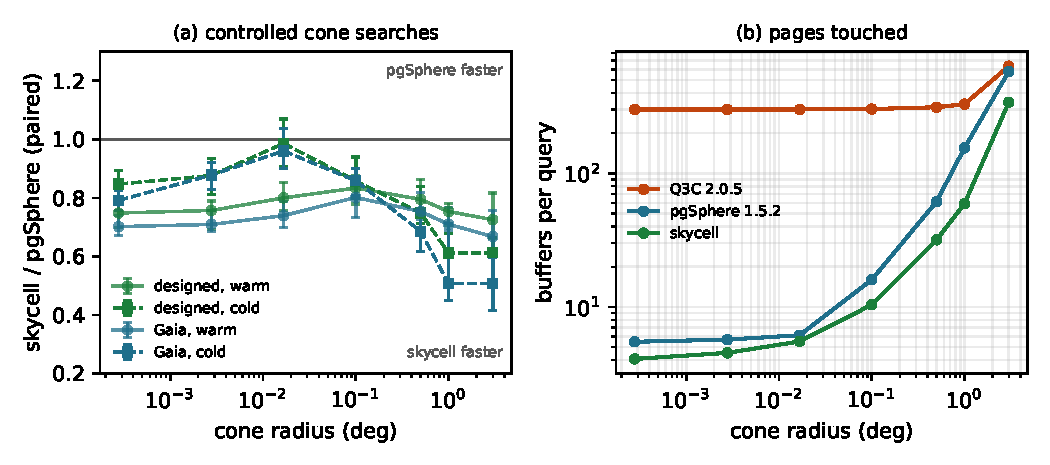
\includegraphics[width=\columnwidth]{fig_benchmark.pdf}
  \caption{\emph{(a)} Paired ratio of \texttt{skycell} to pgSphere against cone radius,
    95\% bootstrap intervals, synthetic corpora, warm and cold; below the line
    \texttt{skycell} is faster. \emph{(b)} Buffer pages touched per query (mean,
    designed corpus).}
  \label{fig:benchmark}
\end{figure}

Table~\ref{tab:cones} and Fig.~\ref{fig:benchmark} give the primary result. Warm,
\texttt{skycell} is faster than pgSphere at every radius on all three corpora, every
interval excluding 1: by 17--33\% on the two synthetic ones and by 4--31\% on real
positions. At 1\arcsec\ it plans in 0.036\,ms against pgSphere's 0.029 and wins in
execution, 0.022\,ms against 0.040, reading 4.1 pages to pgSphere's 5.5. Cold it is
faster or level everywhere: the margin grows with radius to a factor 1.6--2.1 at
1\degr\ and 3\degr, because it touches a third of pgSphere's pages there (59 against 155
on the designed corpus, 85 against 282 on the Gaia one). On real positions it plans in
at most 0.004\,ms more than pgSphere and executes in 0.52--0.82 of its time, reading
fewer pages at every radius; cold, it is faster by a factor 1.5--2.1 from 6\arcmin\ up
and level or slightly faster below, where a first-touch query reads only two or three
pages. On flash storage a saved page is worth about 0.1\,ms; on a slower disk each would
count for more.

Against Q3C, \texttt{skycell} takes 0.02--0.58 of the time, a comparison of
\emph{implementations}: \texttt{q3c\_radial\_query} 2.0.5 expands every call into about
100 bitmap index scans whatever the radius, spending some 2.7\,ms planning them. A
covering-aware radial query in Q3C would close most of that gap;
\Sect~\ref{sec:xmatch} compares the approaches where Q3C carries no such expansion.

\begin{widetable}
  \caption{Cone searches: paired ratio of \texttt{skycell} to pgSphere with its 95\%
    bootstrap interval. Below 1, \texttt{skycell} is faster. \textbf{Bold}: interval
    excludes 1. $n$: distinct queries at that radius. Real corpus: its own centre draw
    at the same radii and counts; cold there uses one table per method and fresh centres,
    so neither method warms the other's pages.}
  \label{tab:cones}
  \centering
  \footnotesize
  \setlength{\tabcolsep}{4pt}
  \begin{tabular}{l r cc cc cc}
    \hline\hline
    & & \multicolumn{2}{c}{designed corpus} & \multicolumn{2}{c}{Gaia corpus (resampled)} & \multicolumn{2}{c}{real Gaia DR3 positions} \\
    \cline{3-4}\cline{5-6}\cline{7-8}
    radius & $n$ & warm & cold & warm & cold & warm & cold \\
    \hline
    1\arcsec  & 400 & \textbf{0.75} [0.70, 0.79] & \textbf{0.85} [0.80, 0.89] & \textbf{0.70} [0.67, 0.74] & \textbf{0.79} [0.76, 0.83] & \textbf{0.83} [0.81, 0.84] & \textbf{0.87} [0.82, 0.94] \\
    10\arcsec & 400 & \textbf{0.76} [0.69, 0.79] & \textbf{0.88} [0.81, 0.94] & \textbf{0.71} [0.68, 0.76] & \textbf{0.88} [0.83, 0.92] & \textbf{0.85} [0.82, 0.86] & 1.01 [0.94, 1.09] \\
    1\arcmin  & 300 & \textbf{0.80} [0.76, 0.85] & 0.99 [0.91, 1.07] & \textbf{0.74} [0.70, 0.79] & 0.96 [0.90, 1.04] & \textbf{0.90} [0.87, 0.92] & 0.98 [0.90, 1.04] \\
    6\arcmin  & 200 & \textbf{0.83} [0.78, 0.88] & \textbf{0.86} [0.80, 0.94] & \textbf{0.80} [0.74, 0.86] & \textbf{0.86} [0.81, 0.90] & \textbf{0.96} [0.93, 0.99] & \textbf{0.61} [0.55, 0.65] \\
    30\arcmin & 100 & \textbf{0.79} [0.75, 0.86] & \textbf{0.75} [0.71, 0.84] & \textbf{0.75} [0.73, 0.82] & \textbf{0.69} [0.62, 0.76] & \textbf{0.81} [0.78, 0.86] & \textbf{0.67} [0.60, 0.72] \\
    1\degr    &  40 & \textbf{0.75} [0.71, 0.78] & \textbf{0.61} [0.52, 0.68] & \textbf{0.71} [0.69, 0.77] & \textbf{0.51} [0.45, 0.72] & \textbf{0.80} [0.75, 0.88] & \textbf{0.53} [0.44, 0.66] \\
    3\degr    &  16 & \textbf{0.73} [0.66, 0.82] & \textbf{0.61} [0.50, 0.66] & \textbf{0.67} [0.63, 0.76] & \textbf{0.51} [0.41, 0.60] & \textbf{0.69} [0.64, 0.75] & \textbf{0.48} [0.43, 0.54] \\
    \hline
  \end{tabular}
\end{widetable}

\subsection{Scale and index size}
\label{sec:scale}
\label{sec:scale-memory}

Ten million rows is 0.55\% of Gaia DR3, so the protocol was repeated at 50 million rows,
where pgSphere's 3439\,MB index exceeds the 2\,GB buffer pool while \texttt{skycell}'s
1071\,MB B-tree still fits (Table~\ref{tab:scale}). Warm, \texttt{skycell} stays 14--31\%
faster at every radius. Cold, its lead grows with size from 30\arcmin\ up, to a factor
1.9 at 30\arcmin, 2.7 at 1\degr\ and 2.4 at 3\degr, as the page gap widens (188 pages
against pgSphere's 642 at 1\degr). Its row estimates stay within a factor 1.3 of the
truth at every radius, where pgSphere's are off by up to 8.7 and Q3C's by up to 2.4.

\begin{table}
  \caption{Paired ratio of \texttt{skycell} to pgSphere on the Gaia density field at two
    catalogue sizes. \textbf{Bold}: interval excludes 1.}
  \label{tab:scale}
  \centering
  \footnotesize
  \begin{tabular}{@{}l cc cc@{}}
    \hline\hline
    & \multicolumn{2}{c}{warm} & \multicolumn{2}{c}{cold} \\
    \cline{2-3}\cline{4-5}
    radius & $10^7$ & $5{\times}10^7$ & $10^7$ & $5{\times}10^7$ \\
    \hline
    1\arcsec  & \textbf{0.70} & \textbf{0.78} & \textbf{0.79} & \textbf{0.82} \\
    10\arcsec & \textbf{0.71} & \textbf{0.78} & \textbf{0.88} & \textbf{0.86} \\
    1\arcmin  & \textbf{0.74} & \textbf{0.86} & 0.96          & 0.98          \\
    6\arcmin  & \textbf{0.80} & \textbf{0.86} & \textbf{0.86} & \textbf{0.81} \\
    30\arcmin & \textbf{0.75} & \textbf{0.75} & \textbf{0.69} & \textbf{0.53} \\
    1\degr    & \textbf{0.71} & \textbf{0.69} & \textbf{0.51} & \textbf{0.37} \\
    3\degr    & \textbf{0.67} & \textbf{0.73} & \textbf{0.51} & \textbf{0.42} \\
    \hline
  \end{tabular}
\end{table}

The per-row index cost is flat between $10^7$ and $5\times10^7$ rows, so it extrapolates
to Gaia DR3's $1.81\times10^9$ sources (Table~\ref{tab:gaia}). The comparison that
matters is between deployments: an archive answering both cone searches and
cross-matches today carries pgSphere plus Q3C, whose \texttt{q3c\_join} is 2.4--2.6
times faster than pgSphere at cross-matching (\Sect~\ref{sec:xmatch}); \texttt{skycell}
answers both, faster, from one index. At DR3 scale that is 38\,GiB against 160\,GiB, the
difference between a 64\,GiB and a 256\,GiB server. Where the buffer pool cannot hold
every index, the smaller one wins: in a 3\,GiB container (768\,MB of shared buffers)
holding a 22\,GB, 20.5-million-row ObsCore-shaped relation, whose GiST index is 1.5
times the pool and \texttt{skycell}'s 0.57 times, \texttt{skycell} answered a stream of
2\degr\ cones sweeping the sky 4.2--4.8 times faster.

\begin{table}
  \caption{Index size and build time at $10^7$ rows, and extrapolated linearly from the
    $5\times10^7$ measurement to Gaia DR3 ($1.81\times10^9$ sources). Last column: the
    smallest conventional server memory holding the index with room for the heap.}
  \label{tab:gaia}
  \centering
  \footnotesize
  \begin{tabular}{@{}l rr rrr@{}}
    \hline\hline
    & \multicolumn{2}{c}{$10^7$ rows} & \multicolumn{3}{c}{at Gaia DR3 scale} \\
    \cline{2-3}\cline{4-6}
    index & MB & build (s) & GiB & build & mem GiB \\
    \hline
    Q3C              & 214 &  5.6 & 38 & 15\,min & 64 \\
    pgSphere         & 685 & 68.6 & 122 & 3.9\,h & 192 \\
    skycell          & 214 &  6.0 & \textbf{38} & 10\,min & 64 \\
    \hline
    pgSphere $+$ Q3C & --- & --- & 160 & 4.1\,h & 256 \\
    \hline
  \end{tabular}
\end{table}

\subsection{Cross-matching and polygons}
\label{sec:xmatch}
\label{sec:otherops}

Cross-matching a user's target list is the operation the Gaia archive lists among its
server-side capabilities and Q3C's own speciality, so it gets the cone searches'
protocol, each method warmed on its own query before timing. On real Gaia DR3 positions,
at the radii cross-matching uses -- optical 1--1.5\arcsec, radio up to 5\arcsec\ -- with
uploads of $10^3$--$10^5$ targets, clustered or uniform (Table~\ref{tab:xmreal}),
\texttt{skycell}'s join is 0.79 of \texttt{q3c\_join}'s time and 0.32 of pgSphere's
over all 24 cells, and faster than both in every one. On the resampled corpus, 200\,000
probes at 1\arcsec\ and 10\arcsec, it is 0.67--0.75 of \texttt{q3c\_join} and 0.26--0.31
of pgSphere, returning the same rows in every trial. The custom scan covers each probe's
cone with the ranges it needs, 1.2 on average at 1\arcsec, reading 4.3 pages per probe.
Written with \texttt{skycell\_cone}, \texttt{skycell\_join} or ADQL's
\texttt{point <@ circle}, the join is the same plan.

Convex polygons of 0.05\degr--2\degr\ take a median 0.28\,ms against pgSphere's 0.77
and Q3C's 1.86, a factor 2.7--4.4 on both synthetic corpora, with pgSphere's tail far
above its median where a polygon's bounding volume fits it poorly. Stored footprints
follow the same pattern: the MOC-in-a-B-tree arrangement answers 200\,474
point-in-region pairs in 0.76\,s against pgSphere's 0.97\,s.

\begin{table}
  \caption{Cross-matching on real Gaia DR3 positions ($10^7$): geometric mean over three
    upload sizes ($10^3$--$10^5$) and two target distributions of the per-cell ratio of
    median times, method order random per cell. \emph{Cone}: the join written with
    \texttt{skycell\_cone}; \emph{join}: with \texttt{skycell\_join}, Q3C's spelling.
    Below 1, \texttt{skycell} is faster; \textbf{bold}: faster in every cell.}
  \label{tab:xmreal}
  \centering
  \footnotesize
  \begin{tabular}{l rr r}
    \hline\hline
    & \multicolumn{2}{c}{vs \texttt{q3c\_join}} & vs pgSphere \\
    \cline{2-3}\cline{4-4}
    radius & cone & join & join \\
    \hline
    $0.5\arcsec$ & \textbf{0.81} & \textbf{0.77} & \textbf{0.30} \\
    $1\arcsec$   & \textbf{0.77} & \textbf{0.76} & \textbf{0.30} \\
    $1.5\arcsec$ & \textbf{0.77} & \textbf{0.78} & \textbf{0.34} \\
    $5\arcsec$   & \textbf{0.84} & \textbf{0.83} & \textbf{0.35} \\
    \hline
    all          & \textbf{0.80} & \textbf{0.79} & \textbf{0.32} \\
    \hline
  \end{tabular}
\end{table}

\subsection{An archive's observation table}
\label{sec:tap}

An ObsCore-shaped relation -- observations in groups of 128 sharing a field centre,
clustered by collection and field -- was built at three sizes from a stored set of field
and query centres drawn from the DR3 density map, and asked the same 30 queries at each
(Table~\ref{tab:crossover}). \texttt{skycell}'s lead grows with the table: by $10^7$
rows it is level on the 0.15\degr\ cone and faster on every other class, 25\% on the
2\degr\ cone, where pgSphere reads 939 pages to its 591. The one class pgSphere wins is
the small cone on the smallest table, where its bitmap scan over field-clustered data
already reads exactly the pages it needs. On a table that small, the database is not
what limits an archive anyway: inside a TAP 1.1 service \citep{egernia} on a
500\,000-row ObsCore corpus, the two indexes tie on throughput at 1--32 concurrent
clients, because the service's own code costs about 10\,ms a request against a fraction
of a millisecond in the database.

\begin{table}
  \caption{ObsCore-shaped relation at three sizes: total query time of \texttt{skycell}
    as the ratio to pgSphere (pgS.), 30 stored centres, two complete randomized runs
    pooled; median buffer pages at $10^7$ rows. Q05: 0.15\degr\ cone; Q06: 2\degr;
    Q07: 0.5\degr\ with calibration and time cuts; Q12: an empty 0.7\arcsec\ cone.}
  \label{tab:crossover}
  \centering
  \footnotesize
  \setlength{\tabcolsep}{3pt}
  \begin{tabular}{l rrr rr}
    \hline\hline
    & \multicolumn{3}{c}{\texttt{skycell} / pgS.} & \multicolumn{2}{c}{buffers, $10^7$} \\
    \cline{2-4}\cline{5-6}
    rows ($10^6$) & 0.5 & 2 & 10 & pgS. & skycell \\
    \hline
    Q05 & 1.14 & 1.07 & 0.97 &  32 &  32 \\
    Q06 & 0.92 & 0.93 & 0.75 & 939 & 591 \\
    Q07 & 0.94 & 0.99 & 0.80 & 113 &  89 \\
    Q12 & 0.71 & 0.68 & 0.47 &   7 &   3 \\
    \hline
  \end{tabular}
\end{table}

\subsection{The density estimate on real positions}
\label{sec:estimator}
\label{sec:ablation}

The cost model reads $\hat\rho$ from Eq.~(\ref{eq:rho}). Table~\ref{tab:estimator}
compares it with $\rho$ counted from the same real-position relation: within 5\% at
Baade's Window and a factor 1.3 at the Galactic pole, low by a factor 10--50 in a
globular cluster core and high by 3.7 at the Galactic centre, as the histogram resolves
a cluster while a query sits inside it and averages it away once the query is larger.
The consequence is smaller than the error: since $s_\star\propto\rho^{-1/2}$, an order
of magnitude in $\rho$ is a factor three in cell size, and the cost curve is flat
across much of that. The covering chosen in a cluster core is within 1.05--1.53 of the
best fixed order, and within 0.98--1.31 where the estimate is accurate, against
243--830 for a fixed order chosen badly: adaptive resolution is worth far more than the
estimate's error costs.

\begin{table}
  \caption{The density estimate $\hat\rho$ against the truth $\rho$ on real Gaia DR3
    positions, radii 0.01\degr--1\degr: median ratio over radii, then over ten
    \texttt{ANALYZE} samples; \emph{samples}: spread of that median across them;
    \emph{range}: over all radii and samples.}
  \label{tab:estimator}
  \centering
  \footnotesize
  \begin{tabular}{l rrr}
    \hline\hline
    field & $\hat\rho/\rho$ & samples & range \\
    \hline
    $\omega$~Cen           & \textbf{0.08} & 0.06--0.09 & 0.05--0.54 \\
    47~Tuc                 & \textbf{0.02} & 0.01--0.11 & 0.00--0.94 \\
    LMC                    & 0.80 & 0.46--0.92 & 0.22--1.26 \\
    Baade's Window         & 0.96 & 0.92--0.98 & 0.45--1.19 \\
    Galactic pole          & 1.27 & 1.18--1.49 & 0.48--1.69 \\
    Galactic centre        & \textbf{3.71} & 3.41--3.80 & 1.95--5.20 \\
    \hline
  \end{tabular}
\end{table}

\subsection{Stored regions}
\label{sec:tests-regions}

On the real 50\,000-row \texttt{fpr} footprint catalogue, the \texttt{float4} box key
beats pgSphere's native GiST on all four region operators (Table~\ref{tab:gistregion}),
and on isolated single-scale bands it reads 10--25\% fewer buffers in 10--20\% less
time; on a mixed circle and polygon corpus the margin widens, since pgSphere needs a
separate index descent per region type.

\begin{table}
  \caption{Region operators on the 50\,000-row \texttt{fpr} catalogue, 500 probes per
    operator: time of the \texttt{float4} box key as the ratio to pgSphere's native
    GiST. Below 1, \texttt{skycell} is faster.}
  \label{tab:gistregion}
  \centering
  \footnotesize
  \begin{tabular}{l r}
    \hline\hline
    operator & box4 / pgSphere \\
    \hline
    \texttt{\&\&} (overlap) & \textbf{0.12--0.17} \\
    \texttt{@>}(region,point) & \textbf{0.75--0.93} \\
    \texttt{@>}(region,region) & \textbf{0.55--0.70} \\
    \texttt{<@}(region,region) & \textbf{0.26--0.27} \\
    \hline
  \end{tabular}
\end{table}

\section{Conclusions}
\label{sec:conclusions}

\texttt{skycell} keeps Q3C's compact integer key and B-tree while answering the region
queries pgSphere was built for, and treats a covering's depth as a cost question --
local source density against the price of an index range -- rather than a constant.
Measured paired against both, it beats each on its own ground. At the cone search,
pgSphere's speciality, it is faster at every radius from 1\arcsec\ to 3\degr\ warm, by
17--33\% on synthetic catalogues and 4--31\% on real Gaia DR3 positions, faster or level
cold, and further ahead as the catalogue grows; it answers convex polygons
2.7--4.4$\times$ faster. At the cross-match, Q3C's speciality, it is 20--33\% faster
than \texttt{q3c\_join} on resampled and real positions alike, and about three times
faster than pgSphere. It does so from an index a third the size of pgSphere's that
builds 11--23 times faster, with one cost parameter derived from the relation's own
statistics, and its region GiST beats pgSphere's on every operator.

The interface matters as much as the speed. \texttt{skycell} speaks ADQL's own
vocabulary, with the indexable \texttt{point <@ circle} answered by the same scan as its
native functions; its stored regions read and write as IVOA STC-S; and one column holds
circles and polygons together, which pgSphere cannot. One compact index serving points,
regions and cross-matches through the language archives already use makes
\texttt{skycell} worth considering as the default positional index of a PostgreSQL
archive, and in particular as a TAP service's geometry layer.

Two limits remain. Planning still costs: a covering is computed per query, so on a
small table a small cone can favour pgSphere (1.14 at $5\times10^5$ rows), and at
1\arcsec\ \texttt{skycell}'s planning, 0.036\,ms, is above pgSphere's 0.029 even as its
execution wins. And the density synopsis is coarse: an equi-depth histogram cannot see a
cluster smaller than a bucket, which the area guard bounds rather than fixes; a stored
multi-order count map is the natural next step.



\section*{CRediT authorship contribution statement}

\textbf{Jes\'us Salgado:} Conceptualization, Methodology, Software, Formal analysis,
Writing -- original draft. \textbf{Michele Delli Veneri:} Validation, Investigation,
Writing -- review \& editing.

\section*{Declaration of competing interest}

The authors declare that they have no known competing financial interests or personal
relationships that could have appeared to influence the work reported in this paper.

\section*{Declaration of generative AI and AI-assisted technologies in the writing process}

During the preparation of this work the authors used Claude Code (Anthropic) in order to
develop the software, the benchmark harness and the analysis, and to draft the
manuscript. After using this tool, the authors reviewed and edited the content as needed
and take full responsibility for the content of the published article. The geometric
predicates and coverings are checked by the brute-force suites of
Section~\ref{sec:validation} against independent computations over millions of
adversarially placed points rather than expected outputs, and every indexed answer in the
regression suites must equal a sequential scan with the exact predicate.

\section*{Data availability}

The extension, its test suites, the benchmark harness and the raw results of every
measurement quoted here are available at
\url{https://github.com/jesusjuansalgado/skycell} under the MIT licence, together with
the history of the measurements that led to the current defaults. All corpora but the
real one are generated from seeds; the real one is drawn from the Gaia archive by a
recorded query.

\section*{Acknowledgements}

This work has made use of data from the European Space Agency (ESA) mission \emph{Gaia}
(\url{https://www.cosmos.esa.int/gaia}), processed by the \emph{Gaia} Data Processing and
Analysis Consortium (DPAC, \url{https://www.cosmos.esa.int/web/gaia/dpac/consortium}).
Funding for the DPAC has been provided by national institutions, in particular the
institutions participating in the \emph{Gaia} Multilateral Agreement.

\section*{Funding}

This research did not receive any specific grant from funding agencies in the public,
commercial, or not-for-profit sectors.

\begin{thebibliography}{}

\bibitem[Chilingarian et al.(2004)]{pgsphere}
Chilingarian, I., Bartunov, O., Richter, J., \& Sigaev, T. 2004,
  in ASP Conf. Ser. 314, Astronomical Data Analysis Software and Systems XIII,
  ed. F. Ochsenbein, M. G. Allen, \& D. Egret (San Francisco: ASP), 225

\bibitem[Delli Veneri \& Salgado(2026)]{egernia}
Delli Veneri, M., \& Salgado, J. 2026, egernia: an IVOA TAP 1.1 server for the SKA
  Observatory, Zenodo, doi:10.5281/zenodo.22845690

\bibitem[Demleitner et al.(2014)]{dachs}
Demleitner, M., Neves, M. C., Rothmaier, F., \& Wambsganss, J. 2014,
  Astron. Comput., 7--8, 27

\bibitem[Dowler et al.(2019)]{tap}
Dowler, P., Rixon, G., Tody, D., \& Demleitner, M. 2019,
  IVOA Recommendation: Table Access Protocol Version 1.1

\bibitem[ESA(1997)]{hipparcos}
ESA 1997, The Hipparcos and Tycho Catalogues, ESA SP-1200

\bibitem[Fernique et al.(2014)]{moc}
Fernique, P., Boch, T., Donaldson, T., et al. 2014,
  IVOA Recommendation: MOC -- HEALPix Multi-Order Coverage map Version 1.0

\bibitem[Gaia Collaboration(2016)]{gaia}
Gaia Collaboration, Prusti, T., de Bruijne, J. H. J., et al. 2016, A\&A, 595, A1

\bibitem[G\'orski et al.(2005)]{healpix}
G\'orski, K. M., Hivon, E., Banday, A. J., et al. 2005, ApJ, 622, 759

\bibitem[Gray et al.(2006)]{zones}
Gray, J., Nieto-Santisteban, M. A., \& Szalay, A. S. 2006,
  The Zones Algorithm for Finding Points-Near-a-Point or Cross-Matching Spatial
  Datasets, Microsoft Research Technical Report MSR-TR-2006-52

\bibitem[Koposov \& Bartunov(2006)]{q3c}
Koposov, S., \& Bartunov, O. 2006, in ASP Conf. Ser. 351, Astronomical Data
  Analysis Software and Systems XV, ed. C. Gabriel, C. Arviset, D. Ponz, \&
  S. Enrique (San Francisco: ASP), 735

\bibitem[Kunszt et al.(2001)]{htm}
Kunszt, P. Z., Szalay, A. S., \& Thakar, A. R. 2001, in Mining the Sky,
  ed. A. J. Banday, S. Zaroubi, \& M. Bartelmann (Berlin: Springer), 631

\bibitem[Moon et al.(2001)]{hilbert}
Moon, B., Jagadish, H. V., Faloutsos, C., \& Saltz, J. H. 2001,
  IEEE Trans. Knowl. Data Eng., 13, 124

\bibitem[Ortiz et al.(2008)]{adql}
Ortiz, I., Lusted, J., Dowler, P., et al. 2008,
  IVOA Recommendation: Astronomical Data Query Language Version 2.0

\bibitem[Rots(2007)]{stc}
Rots, A. H. 2007, IVOA Recommendation: Space-Time Coordinate Metadata for
  the Virtual Observatory Version 1.33

\bibitem[Salgado et al.(2017)]{gaiaarchive1}
Salgado, J., Gonz\'alez-N\'u\~nez, J., Guti\'errez-S\'anchez, R., et al. 2017,
  Astron. Comput., 21, 22

\bibitem[Salgado et al.(2020)]{gaiaarchive2}
Salgado, J., et al. 2020, in ASP Conf. Ser. 522, Astronomical Data Analysis
  Software and Systems XXVII, ed. P. Ballester, J. Ibsen, M. Solar, \&
  K. Shortridge (San Francisco: ASP), 307

\end{thebibliography}


\end{document}
